% Overview figure: build time (a), question time (b), and one worked example (right).
\definecolor{pa}{HTML}{EAF2FB}\definecolor{pad}{HTML}{2F6DB5}
\definecolor{pb}{HTML}{FFF4E5}\definecolor{pbd}{HTML}{C9781B}
\definecolor{pc}{HTML}{F1ECFA}\definecolor{pcd}{HTML}{6B4BB0}
\definecolor{ok}{HTML}{E7F5EA}\definecolor{okd}{HTML}{2E8B57}
\definecolor{hum}{HTML}{FDECEC}\definecolor{humd}{HTML}{C0504D}
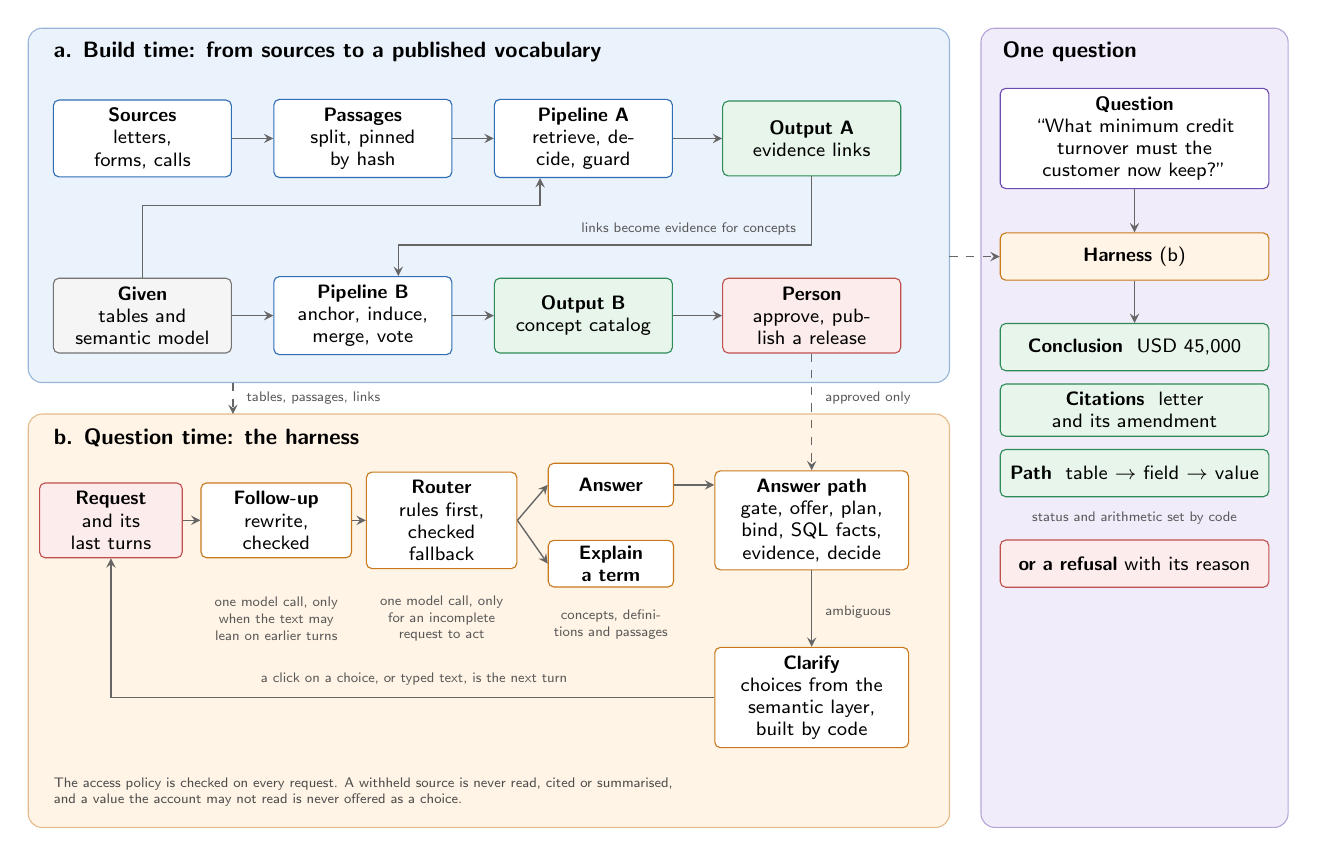
\begin{tikzpicture}[x=1cm,y=1cm,font=\sffamily\scriptsize,>=stealth,
  box/.style={draw=#1,fill=white,rounded corners=2pt,align=center,inner sep=3pt,minimum height=0.95cm,text width=2.05cm},
  box/.default=pad,
  res/.style={box=okd,fill=ok},
  tool/.style={draw=pbd,fill=white,rounded corners=2pt,align=center,inner sep=2pt,minimum height=0.55cm,text width=1.95cm},
  note/.style={align=left,inner sep=2pt,text width=4.95cm,text=black!75},
  arr/.style={->,line width=0.5pt,draw=black!60}]
% panels
\fill[pa,rounded corners=5pt] (0,4.75) rectangle (11.7,9.25);
\draw[pad!50,rounded corners=5pt] (0,4.75) rectangle (11.7,9.25);
\node[anchor=west,font=\sffamily\footnotesize\bfseries] at (0.2,8.95) {a. Build time: from sources to a published vocabulary};
\fill[pb,rounded corners=5pt] (0,-0.9) rectangle (11.7,4.35);
\draw[pbd!50,rounded corners=5pt] (0,-0.9) rectangle (11.7,4.35);
\node[anchor=west,font=\sffamily\footnotesize\bfseries] at (0.2,4.05) {b. Question time: the harness};
\fill[pc,rounded corners=5pt] (12.1,-0.9) rectangle (16.0,9.25);
\draw[pcd!50,rounded corners=5pt] (12.1,-0.9) rectangle (16.0,9.25);
\node[anchor=west,font=\sffamily\footnotesize\bfseries] at (12.25,8.95) {One question};
% a: row 1
\node[box] (src) at (1.45,7.85) {\textbf{Sources}\\letters, forms, calls};
\node[box] (chk) at (4.25,7.85) {\textbf{Passages}\\split, pinned by hash};
\node[box] (pA) at (7.05,7.85) {\textbf{Pipeline A}\\retrieve, decide, guard};
\node[res] (oA) at (9.95,7.85) {\textbf{Output A}\\evidence links};
% a: row 2
\node[box=black!55,fill=black!4] (giv) at (1.45,5.6) {\textbf{Given}\\tables and semantic model};
\node[box] (pB) at (4.25,5.6) {\textbf{Pipeline B}\\anchor, induce, merge, vote};
\node[res] (oB) at (7.05,5.6) {\textbf{Output B}\\concept catalog};
\node[box=humd,fill=hum] (pub) at (9.95,5.6) {\textbf{Person}\\approve, publish a release};
\draw[arr] (src)--(chk); \draw[arr] (chk)--(pA); \draw[arr] (pA)--(oA);
\draw[arr] (pB)--(oB); \draw[arr] (oB)--(pub);
\draw[arr] (oA.south) -- ++(0,-0.87) -| ([xshift=0.45cm]pB.north);
\draw[arr] (giv.north) -- ++(0,0.92) -| ([xshift=-0.55cm]pA.south);
\draw[arr] (giv)--(pB);
\node[font=\sffamily\tiny,text=black!65,anchor=south west] at (6.9,6.5) {links become evidence for concepts};
% a -> b
\node[font=\sffamily\tiny,text=black!65,anchor=west] at (10.0,4.55) {approved only};
\draw[arr,dashed] (2.6,4.75) -- (2.6,4.35);
\node[font=\sffamily\tiny,text=black!65,anchor=west] at (2.65,4.55) {tables, passages, links};
% b
\node[box=humd,fill=hum,text width=1.6cm] (req) at (1.05,3.0) {\textbf{Request}\\and its last turns};
\node[box=pbd,text width=1.7cm] (rw) at (3.15,3.0) {\textbf{Follow-up}\\rewrite, checked};
\node[box=pbd,text width=1.7cm] (rt) at (5.25,3.0) {\textbf{Router}\\rules first, checked fallback};
\node[tool,text width=1.45cm] (t1) at (7.4,3.45) {\textbf{Answer}};
\node[tool,text width=1.45cm] (t2) at (7.4,2.45) {\textbf{Explain a term}};
\node[box=pbd,text width=2.25cm] (ap) at (9.95,3.0) {\textbf{Answer path}\\gate, offer, plan, bind, SQL facts, evidence, decide};
\node[box=pbd,text width=2.25cm] (cl) at (9.95,0.75) {\textbf{Clarify}\\choices from the semantic layer, built by code};
\draw[arr] (req)--(rw); \draw[arr] (rw)--(rt);
\foreach \t in {t1,t2} \draw[arr] (rt.east) -- (\t.west);
\draw[arr] (t1.east)--(ap.west|-t1.east);
\draw[arr] (ap)--(cl);
\draw[arr,dashed] (pub.south) -- (ap.north);
\draw[arr] (cl.west) -- (1.05,0.75) -- (req.south);
\node[font=\sffamily\tiny,text=black!65,anchor=south] at (4.9,0.78) {a click on a choice, or typed text, is the next turn};
\node[font=\sffamily\tiny,text=black!65,anchor=west] at (10.0,1.83) {ambiguous};
\node[font=\sffamily\tiny,text=black!65,align=center,text width=1.95cm] at (3.15,1.75) {one model call, only when the text may lean on earlier turns};
\node[font=\sffamily\tiny,text=black!65,align=center,text width=1.95cm] at (5.25,1.75) {one model call, only for an incomplete request to act};
\node[font=\sffamily\tiny,text=black!65,align=center,text width=1.9cm] at (7.4,1.68) {concepts, definitions and passages};
\node[font=\sffamily\tiny,text=black!70,anchor=west,align=left] at (0.2,-0.45) {The access policy is checked on every request. A withheld source is never read, cited or summarised,\\and a value the account may not read is never offered as a choice.};
% right column
\node[box=pcd,text width=3.2cm] (q) at (14.05,7.85) {\textbf{Question}\\``What minimum credit turnover must the customer now keep?''};
\node[box=pbd,fill=pb,text width=3.2cm,minimum height=0.6cm] (h) at (14.05,6.35) {\textbf{Harness} (b)};
\node[res,text width=3.2cm,minimum height=0.6cm] (r1) at (14.05,5.2) {\textbf{Conclusion}\ \ USD 45,000};
\node[res,text width=3.2cm,minimum height=0.6cm] (r2) at (14.05,4.4) {\textbf{Citations}\ \ letter and its amendment};
\node[res,text width=3.2cm,minimum height=0.6cm] (r3) at (14.05,3.6) {\textbf{Path}\ \ table $\to$ field $\to$ value};
\node[box=humd,fill=hum,text width=3.2cm,minimum height=0.6cm] (r4) at (14.05,2.45) {\textbf{or a refusal} with its reason};
\draw[arr] (q)--(h); \draw[arr] (h)--(r1);
\node[font=\sffamily\tiny,text=black!65] at (14.05,3.03) {status and arithmetic set by code};
\draw[arr,dashed] (11.7,6.35) -- (h.west);
\end{tikzpicture}
